\section{Database og Data Access Layer}\label{sec:designdatabase}

%\subsection{Indledende design overvejelser}
Før design af database og data access layer, er der foretaget nogle indledende tekonologiundersøgelser.

\subsection{Indledende overvejelser}
Fra starten har det været klart at systemet skulle udvikles i flere faser. Databasen og data access laget er derfor udviklet sideløbende med resten af systemets funktionalitet.

Projektets mange iterationer kan deles op i 3 faser, hvor det i første fase var målet at kunne oprette en bruger/User, og også lave forespørgsler på databasen.
DDS-Lite blev brugt i første forsøg med at oprette en funktionel database til at gemme brugere og brugerinformation. Dette viste sig og at være en uholdbar løsning da systemet løbende opdateres. I forbindelse med kurset I4DAB, blev der lavet en opgave hvor Entity Frameworket blev brugt. Dette framework gør det let at udvide systemet, hvilket passer godt til den iterative tilgang der er brugt i projektet. Entity Frameworket er en \textit{Object Relational Mapper}, der gør det lettere at integrere rå data records i et objekt orienteret system. Entity Frameworket gør det med andre ord muligt at behandle rå data records som objekter.

I grove træk vises Entity Frameworkets overordnede virkemåde på figur~\ref{fig:EFarch}, det skal nævnes at ''Application'' på figuren symbolisere data access laget.

\begin{figure}[h]
\centering
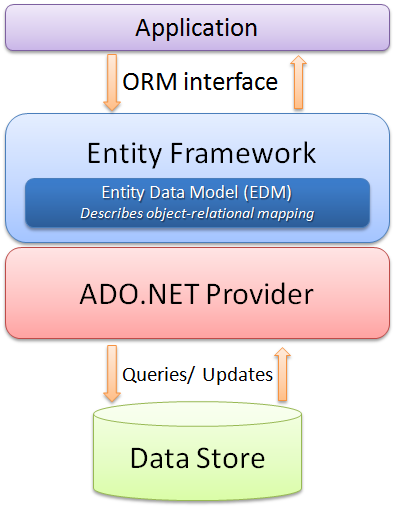
\includegraphics[width=0.5\linewidth]{figs/dbExtra/EFarch}
\caption{Entity Framework \cite{efArch}, hvor ''Application'' på diagrammet er DAL i systemet.}
\label{fig:EFarch}
\end{figure}


Helt fra begyndelsen af databasen og data access lagets designfase, har tanken været at skabe en software komponent, der blot eksponerer et interface, der skal gøre det nemt for klienter at bruge det. Der er lavet et dependancy diagram som kan ses på figur~\ref{fig:vs_codeMap}.

Efter Entity Framkeworket blev vedtaget til brug, blev der udarbejdet et ER diagram ved hjælp af Visual Studio's modelling project. Der er flere måder at designe databaser på i Entity Frameworket. Undervejs er flere af dem blevet afprøvet, herunder \textit{Code First}, \textit{Model First} samt \textit{Database First}.

\textit{Database first} blev brugt i forlængelse med DDS-Lite, som blev brugt til at designe selve databasen. Code First tilgangen gav en bred forståelse for hvordan Entity Frameworket fungerede.

Dog blev \textit{Model First} tilgangen valgt, da der i projektets udviklingsfase ofte blev foretaget markante ændringer i designet. \textit{Model first} gør det lettere at udføre ER opdateringer, direkte på modellen og derefter køre et tilhørende SQL script direkte på databasen. 

Når der skal oprettes en database model, tilføjes der en \textit{ADO.NET Entity Data Model}. Model designeren bruges da til at tilføje, fjerne og ændre i entities.
På figur~\ref{fig:modelDesigner} vises brugen af designeren i projektet.

\begin{figure}
	\centering
	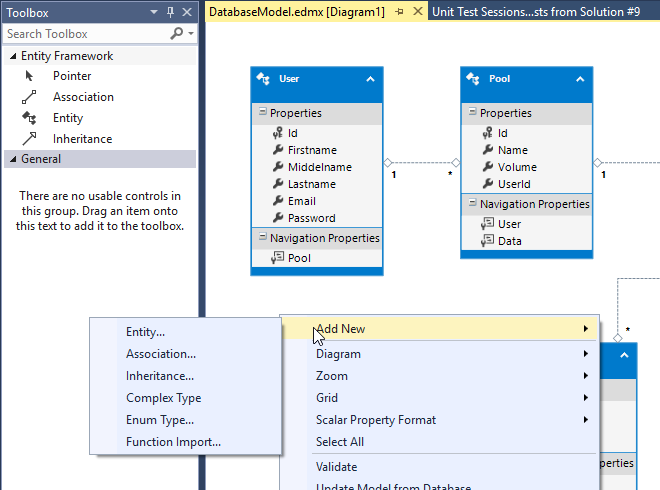
\includegraphics[width=\linewidth]{figs/modelDesigner}
	\caption{Eksempel på entity klasserne i projektet}
	\label{fig:modelDesigner}
\end{figure}

\begin{figure}
\centering
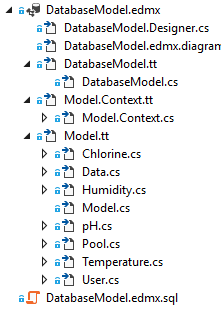
\includegraphics[width=0.35\linewidth]{figs/generatedFiles}
\caption{Eksempel på entity klasserne i projektet}
\label{fig:generatedFiles}
\end{figure}

Nar der udvikles en database med Model First tilgangen, autogenereres de simple entity klasser (User, Pool Data osv.). Dette er klart at foretrække når systemet er under udvikling idet model designeren selv kan opdatere klasserne når modellen opdateres eller udvides. På denne måde undgås det at man selv skal ind og ændre alle entity klasserne manuelt. På figur~\ref{fig:generatedFiles} ses et eksempel på nogen af de autogenerede klasser.

Det første \textit{Model first} udkast til projektets database var meget omfattende og blev lavet før de første rigtige iterationer begyndte. Grunden til at denn emodel blev lavet var at tankegangen med at definere hele systemet fra starten af ikke var "sluppet" helt. Modellen er sidenhen blevet revideret og omkonstrueret. Se figur~\ref{fig:databaseERD_firstattempt_uml} for dette tidlige design.

\begin{figure}[h]
	\centering
	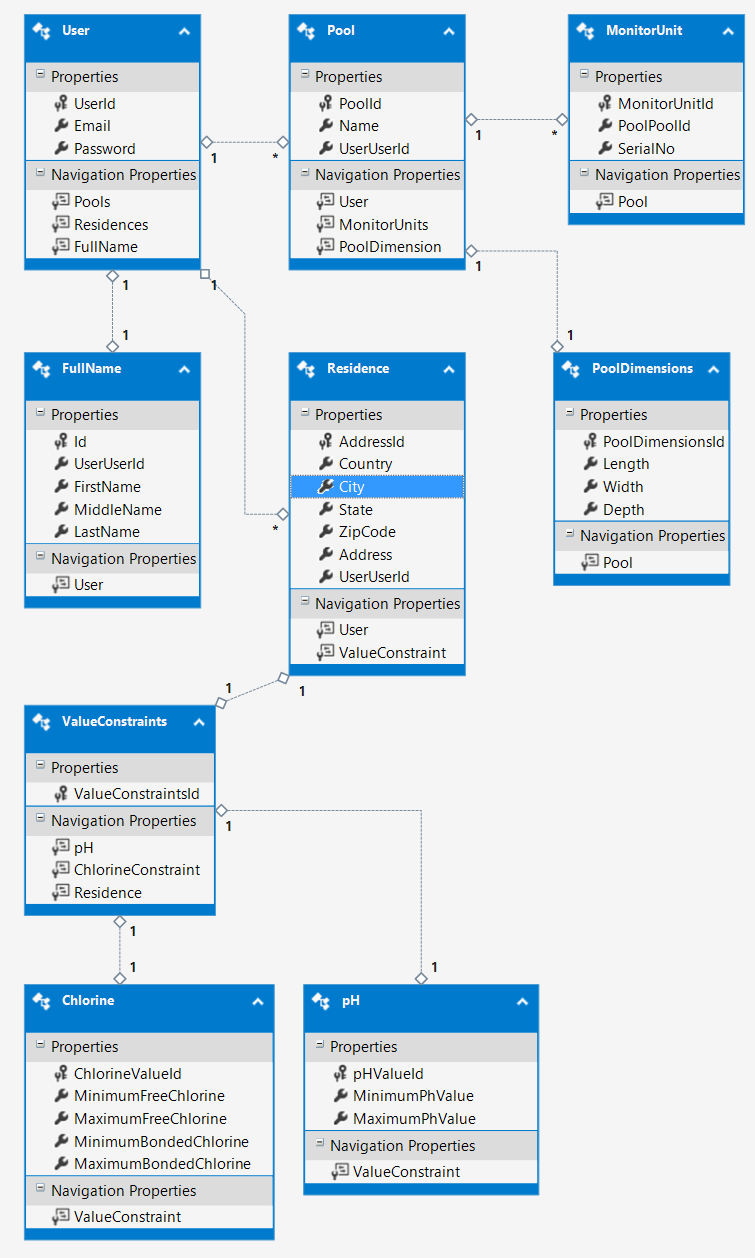
\includegraphics[width=0.8\linewidth]{figs/design/databaseERD}
	\caption{Første "Model First tilgang" til database design}
	\label{fig:databaseERD_firstattempt_uml}
\end{figure}

I løbet af udviklingsprocessen er der foretaget mange ændringer af modellen der ses på figur~\ref{fig:databaseERD_firstattempt_uml}. 
I takt med at man tilegnede sig mere viden omkring database design blev der foretaget flere justeringer. Af markante ændringer kan der nævnes:

\begin{itemize}
	\item FullName entiteten fjernes, User får 3 naming properties.
	\item Residence entiteten fjernes, og Pool entitens \textit{Name} property står for indhold af både addresse og navn.
	\item Value constraints fjernes helt da de ikke er nødvendige at have på databasen
	\item PoolDimensions entiteten fjernes, og Pool får en \textit{Volume} property.
	\item MonitorUnit entiteten udgår af fra databasen. Denne har kun været i databasen for at checke på et evt. serienummer.
	\item Persistering af data er blevet smartere, se figur \ref{fig:databaseERD_final_uml}.
\end{itemize}

\begin{figure}[h]
	\centering
	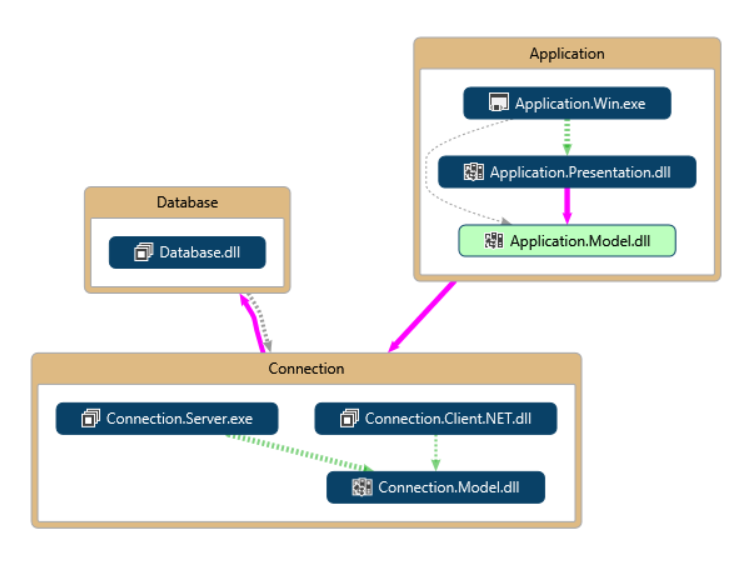
\includegraphics[width=0.8\linewidth]{figs/design/vs_codeMap.PNG}
	\caption{Dependancy graf for Smartpool Systemet}
	\label{fig:vs_codeMap}
\end{figure}

\subsection{User Stories}
Herunder vil databasen og data access lagets funktionalitet blive beskrevet ud fra de undervejs opstillede \textit{user stories}, herunder:

\begin{itemize}
	\item Som bruger vil jeg kunne oprette mig i systemet for at få adgang til systemet.
	\item Som administrator vil jeg kunne slette en bruger for at undgå spild af plads i databasen.
	\item Som bruger vil jeg kunne logge ind i systemet for at se mine data.
	\item Som bruger vil jeg kunne nulstille mit kodeord hvis jeg skulle glemme det.
	\item Som bruger vil jeg skulle ændre mit password for at sikre min konto.
	\item Som bruger vil jeg kunne tilføje en pool til min konto.
	\item Som bruger vil jeg kunne fjerne en pool fra min konto.
	\item Som bruger vil jeg kunne ændre informationer om en eksisterende pool på min konto.
	\item Som bruger vil jeg kunne se en liste over alle mine pools.
	\item Som bruger vil jeg kunne se de seneste sensor værdier for at kunne få et overblik over poolens tilstand.
\end{itemize}

\subsubsection{Oprettelse/ændring af brugere}
Herunder beskrives dokumentation for følgende \textit{user stories}:

\textit{"Som bruger vil jeg kunne oprette mig i systemet for at få adgang til systemet"}

\textit{"Som administrator vil jeg kunne slette en bruger for at undgå spild af plads i databasen"}

\textit{"Som bruger vil jeg kunne logge ind i systemet for at se mine data"}

Ud fra disse user stories, blev det besluttet af en bruger skulle have attributterne som vist på figur~\ref{fig:database_model_1}. Da entiteten er oprettet i databasen som en tabel, skulle data access laget nu designes så \gls{windserver} har adgang til brugerfunktionalitet.


\begin{figure}[H]
	\centering
	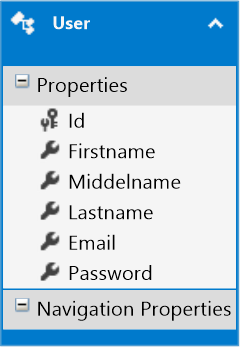
\includegraphics[width=0.25\linewidth]{figs/design/database_model_1}
	\caption{Model for første design for database-adgang.}
	\label{fig:database_model_1}
\end{figure}

Dette blev udviklet med TDD, hvor der først blev skrevet enhedstest som testede følgende scenarier: 

\begin{lstlisting}[caption=Testcases til \textit{AddUser} metoden.,label=code:addusertestcases]
public void AddUser_InsertsUserWith3Names_UserHasCorrectFirstname()
public void AddUser_InsertsUserWith3Names_UserHasCorrectMiddelname()
public void AddUser_InsertsUserWith3Names_UserHasCorrectLastname()
public void AddUser_InsertUserWith2Names_UserHasCorrectFirstname()
public void AddUser_InsertUserWith2Names_UserHasCorrectLastname()
public void AddUser_AddingUserWith1NameOnly_ReturnsFalse()
public void AddUser_InsertUserWithAlreadyUsedEmail_ReturnsFalse()
public void AddUser_InsertUserWithAlreadyUsedEmail_SecondUserIsNotInDatabase()
public void AddUser_Add2UsersWithSameEmailWithDiffCaPiTaL_ReturnsFalse()
\end{lstlisting}

Et eksempel på implementeringen af en testcases, som sikre at der ikke kan sættes en bruger ind med et ''taget'' password, finders herunder. Øvrige testcases med implementering kan se i vedlagt source kode i \textit{Smartpool} solutionen, \textit{Database.Test.Unit} projektet, i \textit{UserAccessUnitTest.cs} filen.

\begin{lstlisting}
...
[Test]
public void AddUser_InsertUserWithAlreadyUsedEmail_ReturnsFalse()
{
	_uut.AddUser("John Johnson", "mail", "password");
	
	Assert.That(_uut.AddUser("Derp Derpsen", "mail", "wordpass"), Is.False);
}
...
\end{lstlisting}

Disse blev udfærdiget og implementeret. Undervej blev der selvfølgelig fundet fejl i både test og kode, men tiden brugt på at rette fejlene på dette tidspunkt blev vurderet til at være væsentligt kortere end hvis de først blev fundet senere i processen. 

Endeligt kom \textit{AddUser} metoden til at se ud som vist på listing~\ref{code:adduser} og på grund af TDD er det med en test-coverage på 100\%.

\begin{lstlisting}[caption=\textit{AddUser} klassen,label=code:adduser]
public bool AddUser(string fullname, string email, string password)
{
	if (IsEmailInUse(email)) return false;
	if (!ValidateName(fullname)) return false;
	
	User user;
	
	string[] names = fullname.Split(' ');
	
	if (names.Length <= 2)
	{
		user = new User() { Firstname = names[0], Lastname = names[1], Email = email, Password = password };
	}
	else
	{
		user = new User() { Firstname = names[0], Middelname = names[1], Lastname = names[2], Email = email, Password = password };
	}
	
	using (var db = new DatabaseContext())
	{
		db.UserSet.Add(user);
		db.SaveChanges();
	}
	
	return true;
}
\end{lstlisting}

Da metoden til at sætte en bruger ind i databasen med DAL var skrevet og testet, skulle der implementeres funktionalitet til at hente denne bruger ud af databasen. Til dette blev følgende testcases designet:

\begin{lstlisting}[caption=Testcases til \textit{FindUserByEmail} metoden.,label=code:finduserbyemailtestcases]
public void FindUserByEmail_UserIsNotAdded_ReturnsNullUser()
public void FindUserByEmail_UserIsAdded_FindsCorrectUser()
public void FindUserByEmail_TwoUsersWithSameEmailInDB_ThrowsMultipleEmailsFoundException()
public void FindUserByEmail_InsertsUserWithEmailInAllCaps_FindUserSearchingWithLowerCaps()
\end{lstlisting}

Dette er lavet efter samme fremgangsmåde som beskrevet med \textit{AddUser} metoden. Sådan er funktionaliteten til at finde en bruger udviklet og på grund af dette igen med fuldstændigt testcoverage. Metoden er vist herunder: 

\begin{lstlisting}
public User FindUserByEmail(string email)
{
	User foundUser;
	
	using (var db = new DatabaseContext())
	{
		var searchByEmail = from search in db.UserSet
		where search.Email.Equals(email)
		select search;
	
		if (searchByEmail.Count() > 1) 
			throw new MultipleOccourencesOfEmailWasFoundException();
		if (searchByEmail.Count() == 0) 
			throw new UserNotFoundException();
	
		foundUser = searchByEmail.First();
	}
	
	return foundUser;
}
\end{lstlisting}

Da \textit{FindUserByEmail} skal returnere en instans af \textit{User} klassen, var der begrænset mulighed for at gøre ''kalder'' klar over at en fejl var forekommet. Så \textit{FindUserByEmail} kaster en exception hvis det ikke går godt.

Endeligt var der behov for at kunne verificere en brugers password. I forbindelse med dette var det vigtigt at selve kodeordet aldrig forlader data access laget. Måden det blev implementeret på var at brugeren af metoden måtte sende email og kodeord med som argument, hvorefter \textit{ValidatePassword} skulle svare om disse matchede. Igen blev der fundet en række testcases:

\begin{lstlisting}[caption=Testcases til \textit{ValidatePassword} metoden.,label=code:validatepasswordtestcases]
public void ValidatePassword_ValidPassword_ReturnsTrue()
public void ValidatePassword_InvalidPassword_ReturnsFalse()
public void ValidatePassword_UserIsNotInDB_ReturnsFalse()
\end{lstlisting}

Disse blev skrevet og løbende blev \textit{ValidatePassword} implementeret, som vist herunder:

\begin{lstlisting}
public bool ValidatePassword(string email, string password)
{
	User user;
	try
	{
		user = FindUserByEmail(email);
	}
	catch (Exception e)
	{
		Console.WriteLine("Herro pree, u can haz exception: " + e);
		return false;
	}
	
	if (user.Password == password) return true;
	
	return false;
}
\end{lstlisting}

\subsubsection{Nulstilling/ændring af password}
Herunder beskrives dokumentation for følgende \textit{user stories}:

\textit{"Som bruger vil jeg kunne nulstille mit kodeord hvis jeg skulle glemme det"}

\textit{"Som bruger vil jeg skulle ændre mit password for at sikre min konto"}

For at en bruger kan ændre sit password, skal der på User entiteten være en property til et kodeord, er allerede indsat på figur~\ref{fig:database_model_1}















For at lave dette på en måde som gjorde udvidelse let, kom første udkast til at se ud som vist på figur~\ref{fig:database_class_1}. Adgangen til databasen skulle være simpel. Dette var på grund af grænsefladen til resten af system, som skulle udvikles samtidigt. På denne måde skulle de øvrige grupper ikke ændre deres brug af \textit{ISmartpool} interfacet.  Derfor skulle der laves én klasse som ville have associationer til specialiserede klasser. Figur~\ref{fig:database_class_1} viser hvordan kaldet fra \textit{context} går gennem klassen \textit{ISmartpool}.

\begin{figure}[h]
	\centering
	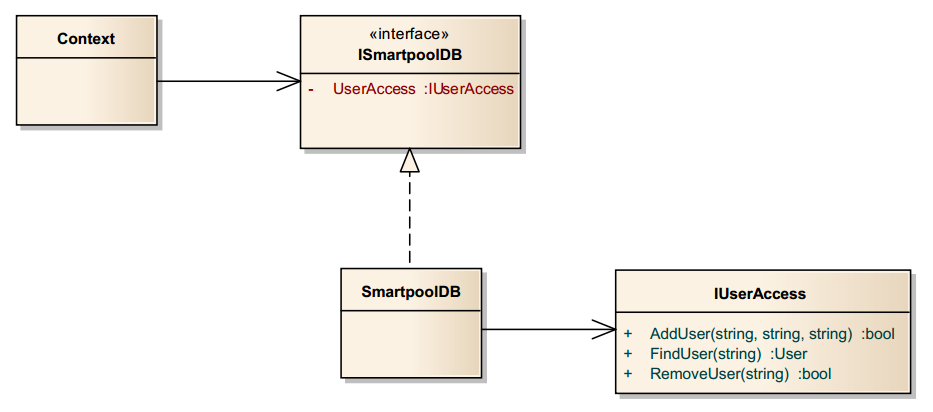
\includegraphics[width=0.9\linewidth]{figs/design/database_class_1}
	\caption{Første design for database-adgang.}
	\label{fig:database_class_1}
\end{figure}

På denne måde skulle \textit{UserAccess} klasse så stå for adgang til brugerinformationer i databasen. 

Der skulle så laves en simple database, med det eneste formål at kunne indeholde disse basale informationer om brugerne af systemet.

\begin{itemize}
	\item Navn (for, mellem og -efternavn)
	\item Email
	\item Password
\end{itemize}

Med \gls{ef} blev følgende model lavet til at opfylde dette krav.

Udfra dette blev et script genereret, som så skulle køres mod en localdb. Nu var databasen oprettet og implementeringen af \textit{UserAccess} klassen kunne starte.

\subsection{Persistering af sensordata}
%Husk at tage udgangspunkt historisk pool data US
Da Smartpool systemet kræver lagring af større mængder data er der gjort en del overvejelser på området. 
En tidlig udgave af database designet kan ses på figir~\ref{fig:databaseERD_final_uml}. Her gemmes alt indsamlet data i én stor tabel. Dette er uhensigtsmæssigt i forbindelse med data queries, da der på denne måde skulle søges i et meget større dataset end nødvendigt. Designet er siden blevet optimeret. 

Ser man på figur~\ref{fig:databaseERD_final_uml}, er entiteten MonitorUnit blevet fjernet. Dataen ligger her i hver sin respektive tabel med henblik på type. Der er tilføjet en Data entitet der har et timestamp som attribut. Man kan derved finde tidsspecfik data, blot ved at kende den Data entitet der kender til brugerens pool. På denne måde er søgetiden optimeret med en faktor 4. Dog vil søgetider stadig blive længere jo flere pools der tilføjes i systemet.

En videre optimering ville være at oprette nye data tabeller hver gang der oprettes en pool i systemet. Dette vil mindske søgetider drastisk. Gruppen har talt med Jesper Tørresø om dette problem, men ingen løsning blev fundet.

Envidere kan data der er ældre end x antal dage, flyttes til en anden tabel. På denne måde vil der komme et max for søgetider i nyere data.
Mulighederne for dette er undersøgt, dog vil løsningen kræve yderligere teknologiundersøgelser, samt tage for lang tid at implementere det nuværende design.

\subsubsection{User Story - Se pooldata}

"\textit{Som bruger vil jeg kunne se mine pooldata.}"\todo{Ændr denne US???}

Det endelige design tillader en bruger at hente sine egen pooldata.

Funktionaliteten hertil er implementeret i projektets data access layer. Udadtil har DAL et interface \textit{ISmartpoolDB} som en klient, \gls{windserver}, kan kalde ind i. Dette er smart da data-access klienten ikke behøves at have referencer til alle DAL klasser.

\begin{lstlisting}[caption=TokenMsgResponse constructor,label=code:tokenMsgRespone_constructor]
public TokenMsgResponse(ISmartpoolDB smartpoolDb)
{
	_smartpoolDb = smartpoolDB;
	...
}
\end{lstlisting}

Som det kan ses på kodeudsnit~\ref{code:tokenMsgRespone_constructor}, initialiseres objektet i klientens constructor.
For at få data trukket ud af databasen kaldes DAL's DataAccess klasse som implementerer DataAccess interfacet IDataAccess. DataAccess har de nødvendige data getter metoder. 
Alle getData metoder returnerer en liste af tupler. Tuplerne indeholder enum SensorTypes, som beskriver hvilken sensor der har foretaget målingen, og en double der repræsenterer målingens værdi.

\begin{lstlisting}[caption=something, label=code:derp]
private List<Tuple<SensorTypes, List<double>>> GetSensorValues(string userName, string poolName, int days)
{
	return new List<Tuple<SensorTypes, List<double>>>
		{
			GetData(_smartpoolDb.DataAccess.GetTemperatureValues(userName, poolName, days), SensorTypes.Temperature),
			GetData(_smartpoolDb.DataAccess.GetPhValues(userName, poolName, days), SensorTypes.Ph),
			GetData(_smartpoolDb.DataAccess.GetChlorineValues(userName, poolName, days), SensorTypes.Chlorine),
			GetData(_smartpoolDb.DataAccess.GetHumidityValues(userName, poolName, days), SensorTypes.Humidity)
		};
}
\end{lstlisting}\todo{missing caption!}

\begin{figure}[h]
	\centering
	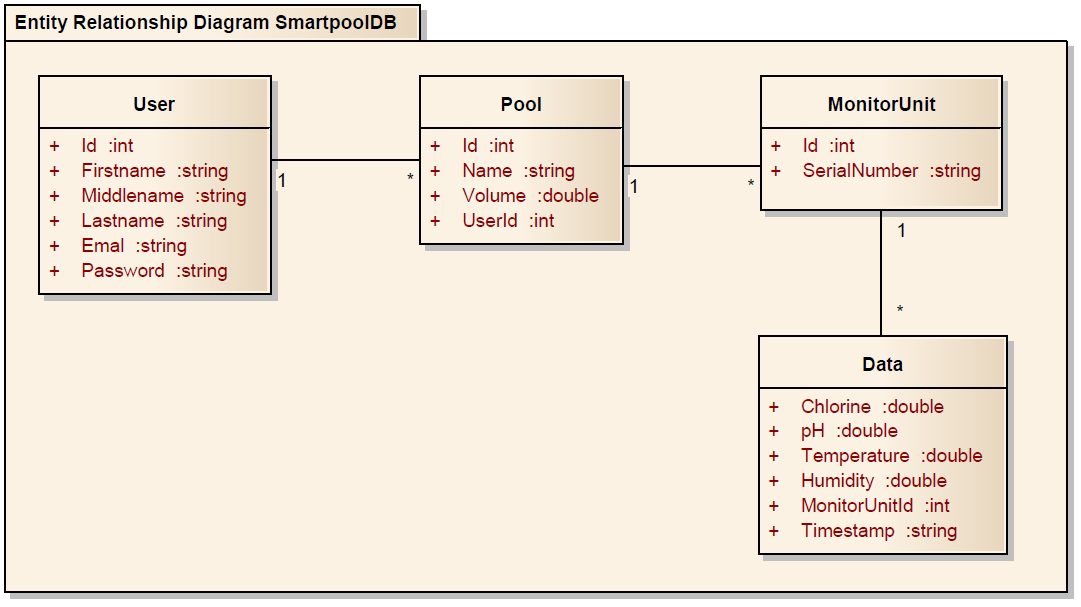
\includegraphics[width=\linewidth]{figs/design/databaseERD_old_uml}
	\caption{Første udgave af ER diagram, UML notation}
	\label{fig:databaseERD_old_uml}
\end{figure}

Sensor data persisteres i hver sin tabel.

\subsection{Endeligt database og DAL design}

\begin{figure}[h]
	\centering
	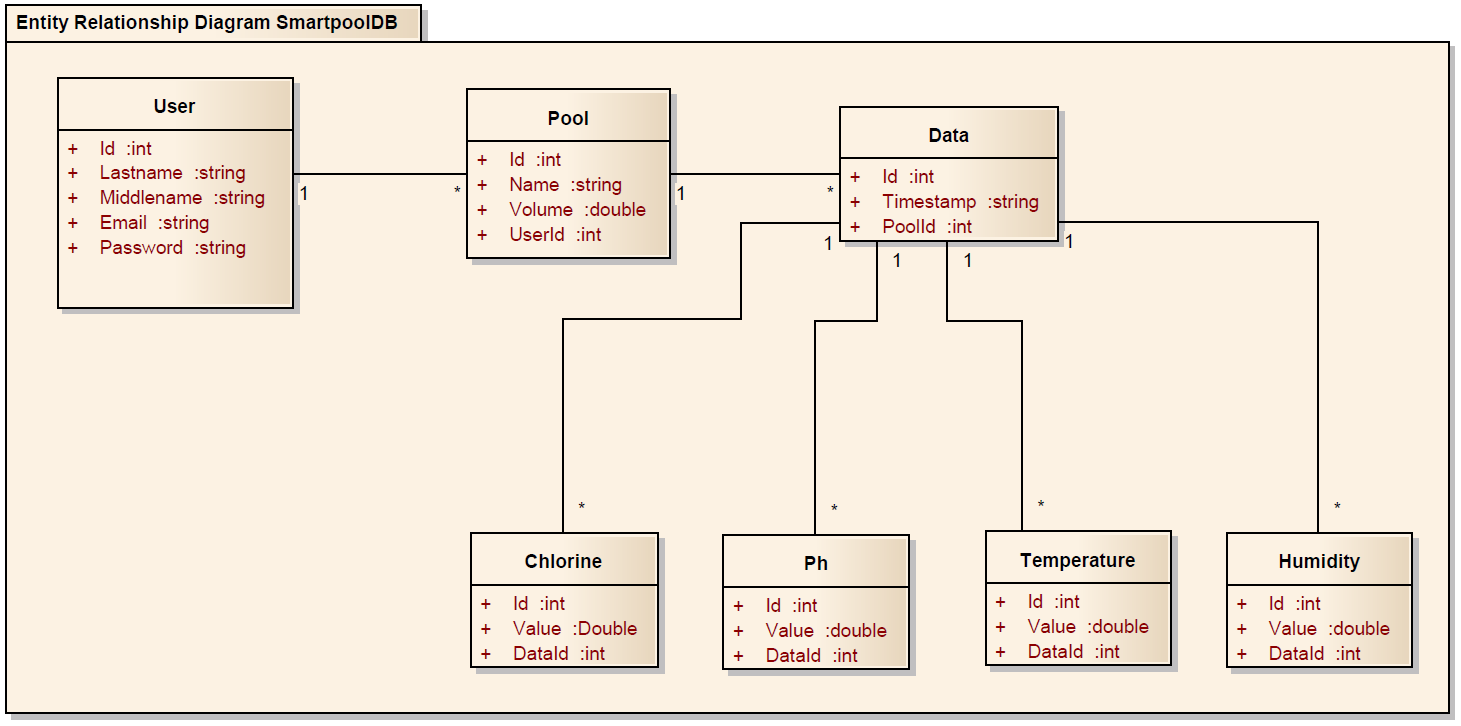
\includegraphics[width=\linewidth]{figs/design/databaseERD_final_uml}
	\caption{Endeligt ER diagram, UML notation}
	\label{fig:databaseERD_final_uml}
\end{figure}

Det endelige database design kan ses på figur~\ref{fig:databaseERD_final_uml}. I modsætning til designet på figur~\ref{fig:databaseERD_firstattempt_uml} er dette design mere simpelt og langt bedre optimeret. Optimeringen ligger til dels i at nogle af entiteterne er samlet til én enkelt, og dels i måden hvorpå data kan hentes ud af databasen. 

\todo{Skriv noget om hvordan man querier på DB her! + noget om hvordan data-pH/chlorine relationen fungerer}

I det nuværende design kan der laves en query på pooldata ved at kalde data getter metoderne i DataAccess klassen. Som det kan ses på figur \ref{fig:getDataClassDiagramPNG} eksponerer DataAccess et interface, IDataAccess der initialiseres i SmartPoolDB klassens constructor.


\begin{figure}[h]
	\centering
	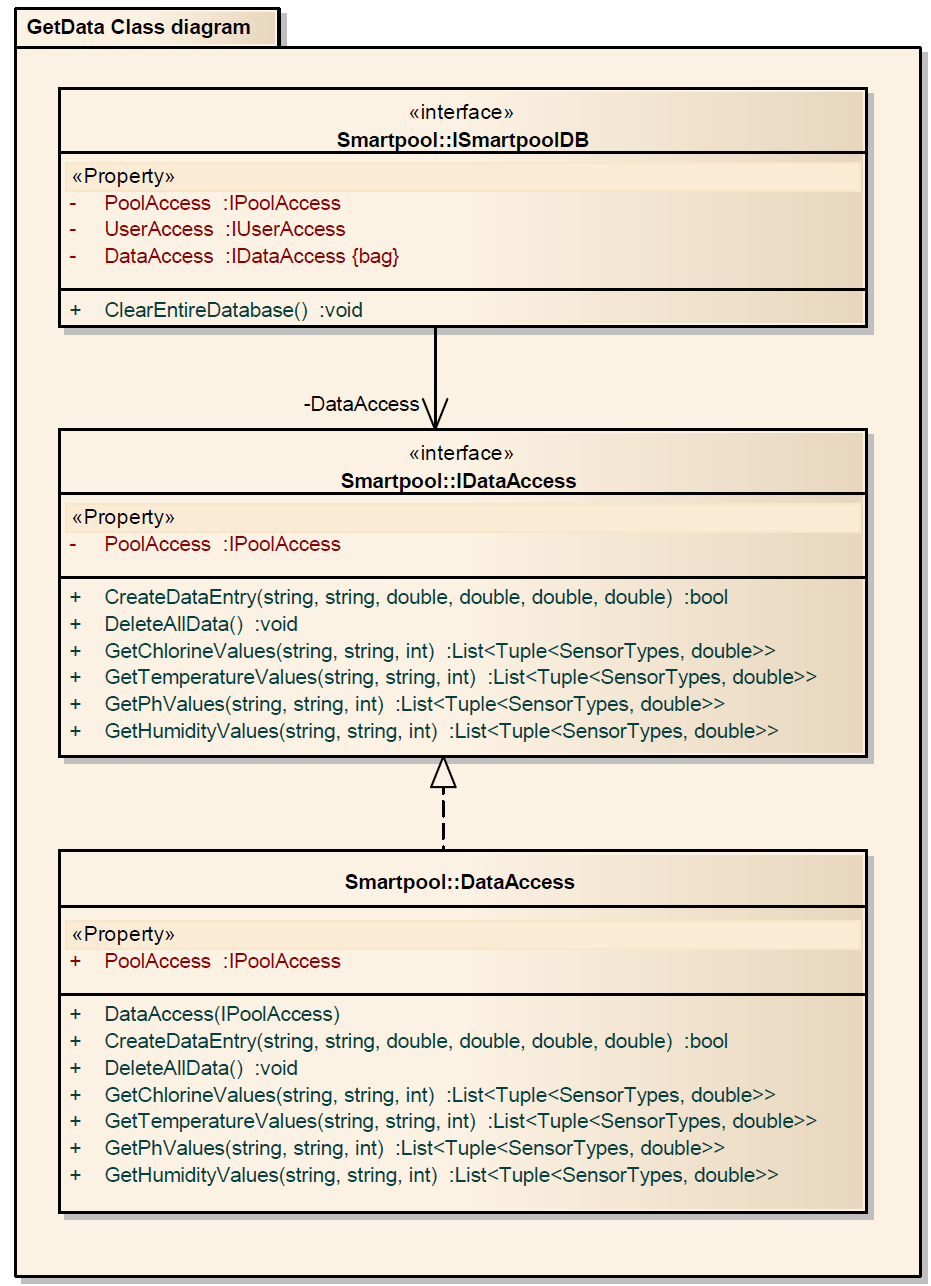
\includegraphics[width=0.7\linewidth]{figs/design/getDataClassDiagramPNG.PNG}
	\caption{Udtag pooldata fra databasen - DataAccess klassediagram}
	\label{fig:getDataClassDiagramPNG}
\end{figure}

Dette designvalg er taget for at simplificere brugen GetData metoder, og for at dependancy inverte forholdet mellem SmartPoolDB og DataAccess. 

\todo{Skriv om DataAcces og IDataAccess}



